\documentclass[aspectratio=169,xcolor=table,10pt]{ctexbeamer}
% \documentclass[aspectratio=169,draft]{ctexbeamer}
% \documentclass[aspectratio=169,handout]{ctexbeamer}
% \documentclass[aspectratio=169,handout,draft]{ctexbeamer}
% \usepackage{pgfpages}
% \pgfpagesuselayout{4 on 1}[a4paper,border shrink=5mm,landscape]
% \setbeameroption{show notes}

\usetheme{Warsaw}
\linespread{1.3}
\useoutertheme{infolines}
\useoutertheme[subsection=false]{smoothbars}
\usecolortheme{SEU}


\title{\textbf{东大信息beamer模板(非官方)}}
\subtitle{\normalfont \itshape 硕~士~学~位~论~文~答~辩}
\author[王东南]{答辩人:\textbf{王东南}\hspace*{3pt} \\指导老师:\textbf{王东}~教授}
\institute[指导老师: 王东~教授]{东南大学 移动通信全国重点实验室\\通信工程(含宽带网络、移动通信等)}
\date{\today}
% \date{2022年12月19日}
\graphicspath{{./}{./img/}{./fig/}{./image/}{./figure/}{./picture/}{../image/}{./SEU_RADIO_image}}
\usepackage{url}
\usepackage{graphicx}  % 插图
\usepackage{float} 
% \usepackage{subfigure}
\usepackage{subfig}
\newcommand{\upcite}[1]{\textsuperscript{\textsuperscript{\cite{#1}}}}
\usepackage[OT1]{fontenc}
\usepackage{cmbright}
\usepackage{sansmathfonts}
% \renewcommand{\sfdefault}{cmss}
% \usefonttheme[onlylarge]{structurebold}
% \setCJKmainfont[ItalicFont={江城斜宋体 300W}]{思源宋体}
\setCJKsansfont{更纱黑体}[
    Path = ./fonts/, 
    UprightFont = sarasa-ui-sc-regular.ttf, % 直立体
    BoldFont = sarasa-ui-sc-bold.ttf,       % 粗体
    ItalicFont = LXGWWENKAI-REGULAR.TTF,    % 斜体
    BoldItalicFont = LXGWWENKAI-BOLD.TTF,   % 粗斜体
] 
% \setCJKmonofont{思源等宽}
% \newcommand{\XWWK}{\CJKfontspec{./fonts/LXGWWENKAI-REGULAR.TTF}}
\newCJKfontfamily\XWWK{霞鹜文楷}[
    Path = ./fonts/, 
    UprightFont = LXGWWENKAI-REGULAR.TTF, % 直立体
    BoldFont = LXGWWENKAI-BOLD.TTF,   % 粗体
    ]
\usepackage{multicol}

% \usepackage{listings}
% \def\lstbasicfont{\ttfamily\selectfont\footnotesize}
% \lstset{%
%    numbers=none,
%    numberstyle=\tiny\sffamily,%
%     showstringspaces=false,
%     showspaces=false,%
%     tabsize=4,%
%     breaklines=true,%
%     frame=lines,%
%     basicstyle={\scriptsize\ttfamily},%
%     keywordstyle=\color{blue},%
%     identifierstyle=,%
%     commentstyle=\itshape\color{teal},%\itshape,%
%     stringstyle=\color{violet},%
%     escapeinside=``,%
%     backgroundcolor=\color[RGB]{245,245,244},
% }
% \lstloadlanguages{C,C++,Java,Matlab,Mathematica,vhdl}
\usepackage{longtable,multirow,array}  % 各种基本的表格宏包
\usepackage{booktabs}  % 三线表宏包
\usepackage{tabularx}
\usepackage{longtable}
\usepackage{tabu}
\usepackage{threeparttable}
% \usepackage{animate}
% \usepackage{wrapfig}
\newcommand{\llra}{\longleftrightarrow}
\newcommand{\rd}{\mathrm{d}}
\newcommand{\Good}{{\color{green}$\blacktriangle$}}
\usepackage{tikz}
\usepackage{pgfplots}
\pgfplotsset{compat=newest}
%% the following commands are needed for some matlab2tikz features
\usetikzlibrary{plotmarks}
\usetikzlibrary{arrows.meta}
\usepgfplotslibrary{patchplots}
\usepackage{tikz}
\usetikzlibrary{positioning, fit, calc}   
\usepackage{xcolor}  
\tikzset{block/.style={draw, thick, text width=1.4cm , minimum height=0.8cm, align=center},   
line/.style={-latex}     
}  
\usepackage{fancybox}
\usepackage{mathrsfs}
\usepackage{mathtools}
\usepackage{annotate-equations}

% \definecolor{XDUcolor}{HTML}{b0252a} %西电红
% \definecolor{XDUcolor}{HTML}{004181} %西电蓝
\renewcommand{\emph}[1]{{\XWWK \structure{#1}}}
% \newcommand{\frametitleb}[1]{\frametitle{\bfseries #1}}
\newcommand{\frametitleb}[1]{\frametitle{\makebox[\framewidth]{\bfseries #1 \hfill\raisebox{-1.5ex}{
\includegraphics[height=1.1\baselineskip]{logo.pdf}}}}}
% \setbeamertemplate{frametitle}
% {
%     \begin{beamercolorbox}[wd=\paperwidth]{frametitle}
%       \strut\hspace{0.5em}\insertframetitle\strut
%       \hfill
%       \raisebox{-2mm}{
\includegraphics[height=1cm]{logo.pdf}}
%     \end{beamercolorbox}
% }
\renewcommand{\thefootnote}{[\arabic{footnote}]}
\newcommand{\bibart}[1]{{\textsuperscript{\textsuperscript{\color{XDUcolor}#1}}}}
\newcommand{\figtext}[3]{\begin{minipage}[t]{.6\textwidth}  \vspace{-15pt}#1 \end{minipage} \begin{minipage}[t]{.35\textwidth}  \begin{exampleblock}{}  \raisebox{-1pt}{\structure{\faArrowCircleLeft}}\parbox{.95\textwidth}{\centering #3}  \end{exampleblock} \pause#2\end{minipage}}
\newcommand{\bs}{\boldsymbol}
\newcommand{\mb}{\mathbf}
% \usepackage[ruled,vlined]{algorithm2e}
\usepackage{fontawesome5}
\newcommand{\NOTICE}{\structure{\bfseries\faMixcloud~注意} }
\newcommand{\emphbf}[1]{\structure{\bfseries#1}}
% \logo{
\includegraphics[height=0.15\textwidth]{logo.pdf}}
% \AtBeginSection[]
% {
%   \begin{frame}<beamer>
%     \frametitle{\textbf{目录}}
%     \tableofcontents[currentsection]
%   \end{frame}
% }

%% 定义节标题页面
\AtBeginSection[]{
    %  \let\insertsectionnumber\relax
     \let\sectionname\relax
     \frame{\sectionpage}
}
\renewcommand{\thesection}{\Roman{section}}
\setbeamertemplate{section page}
{
    \begin{centering}
        {\usebeamerfont{section title} \textsc{Part} \thesection}

        \vspace{10pt}
    \begin{beamercolorbox}[sep=12pt,center,colsep=-4bp,rounded=true,shadow=true]{part title}
    \usebeamerfont{section title}\bfseries\insertsection\par
    \end{beamercolorbox}

    \vspace{20pt}\begin{minipage}
        {.35\linewidth}
        \tableofcontents[sectionstyle=hide,subsectionstyle=show/shaded/hide]
    \end{minipage}
    
    \end{centering}
}

%% 定义小节标题页面
% \AtBeginSubsection[]
% {
% \begin{frame}[shrink]

%     \centering
%         \tableofcontents[sectionstyle=show/shaded,subsectionstyle=show/shaded/hide]

% \end{frame}
% }

%% 标题页样式
\titlegraphic { 
\begin{tikzpicture}[overlay,remember picture]
\node[above left] at (current page.332){
    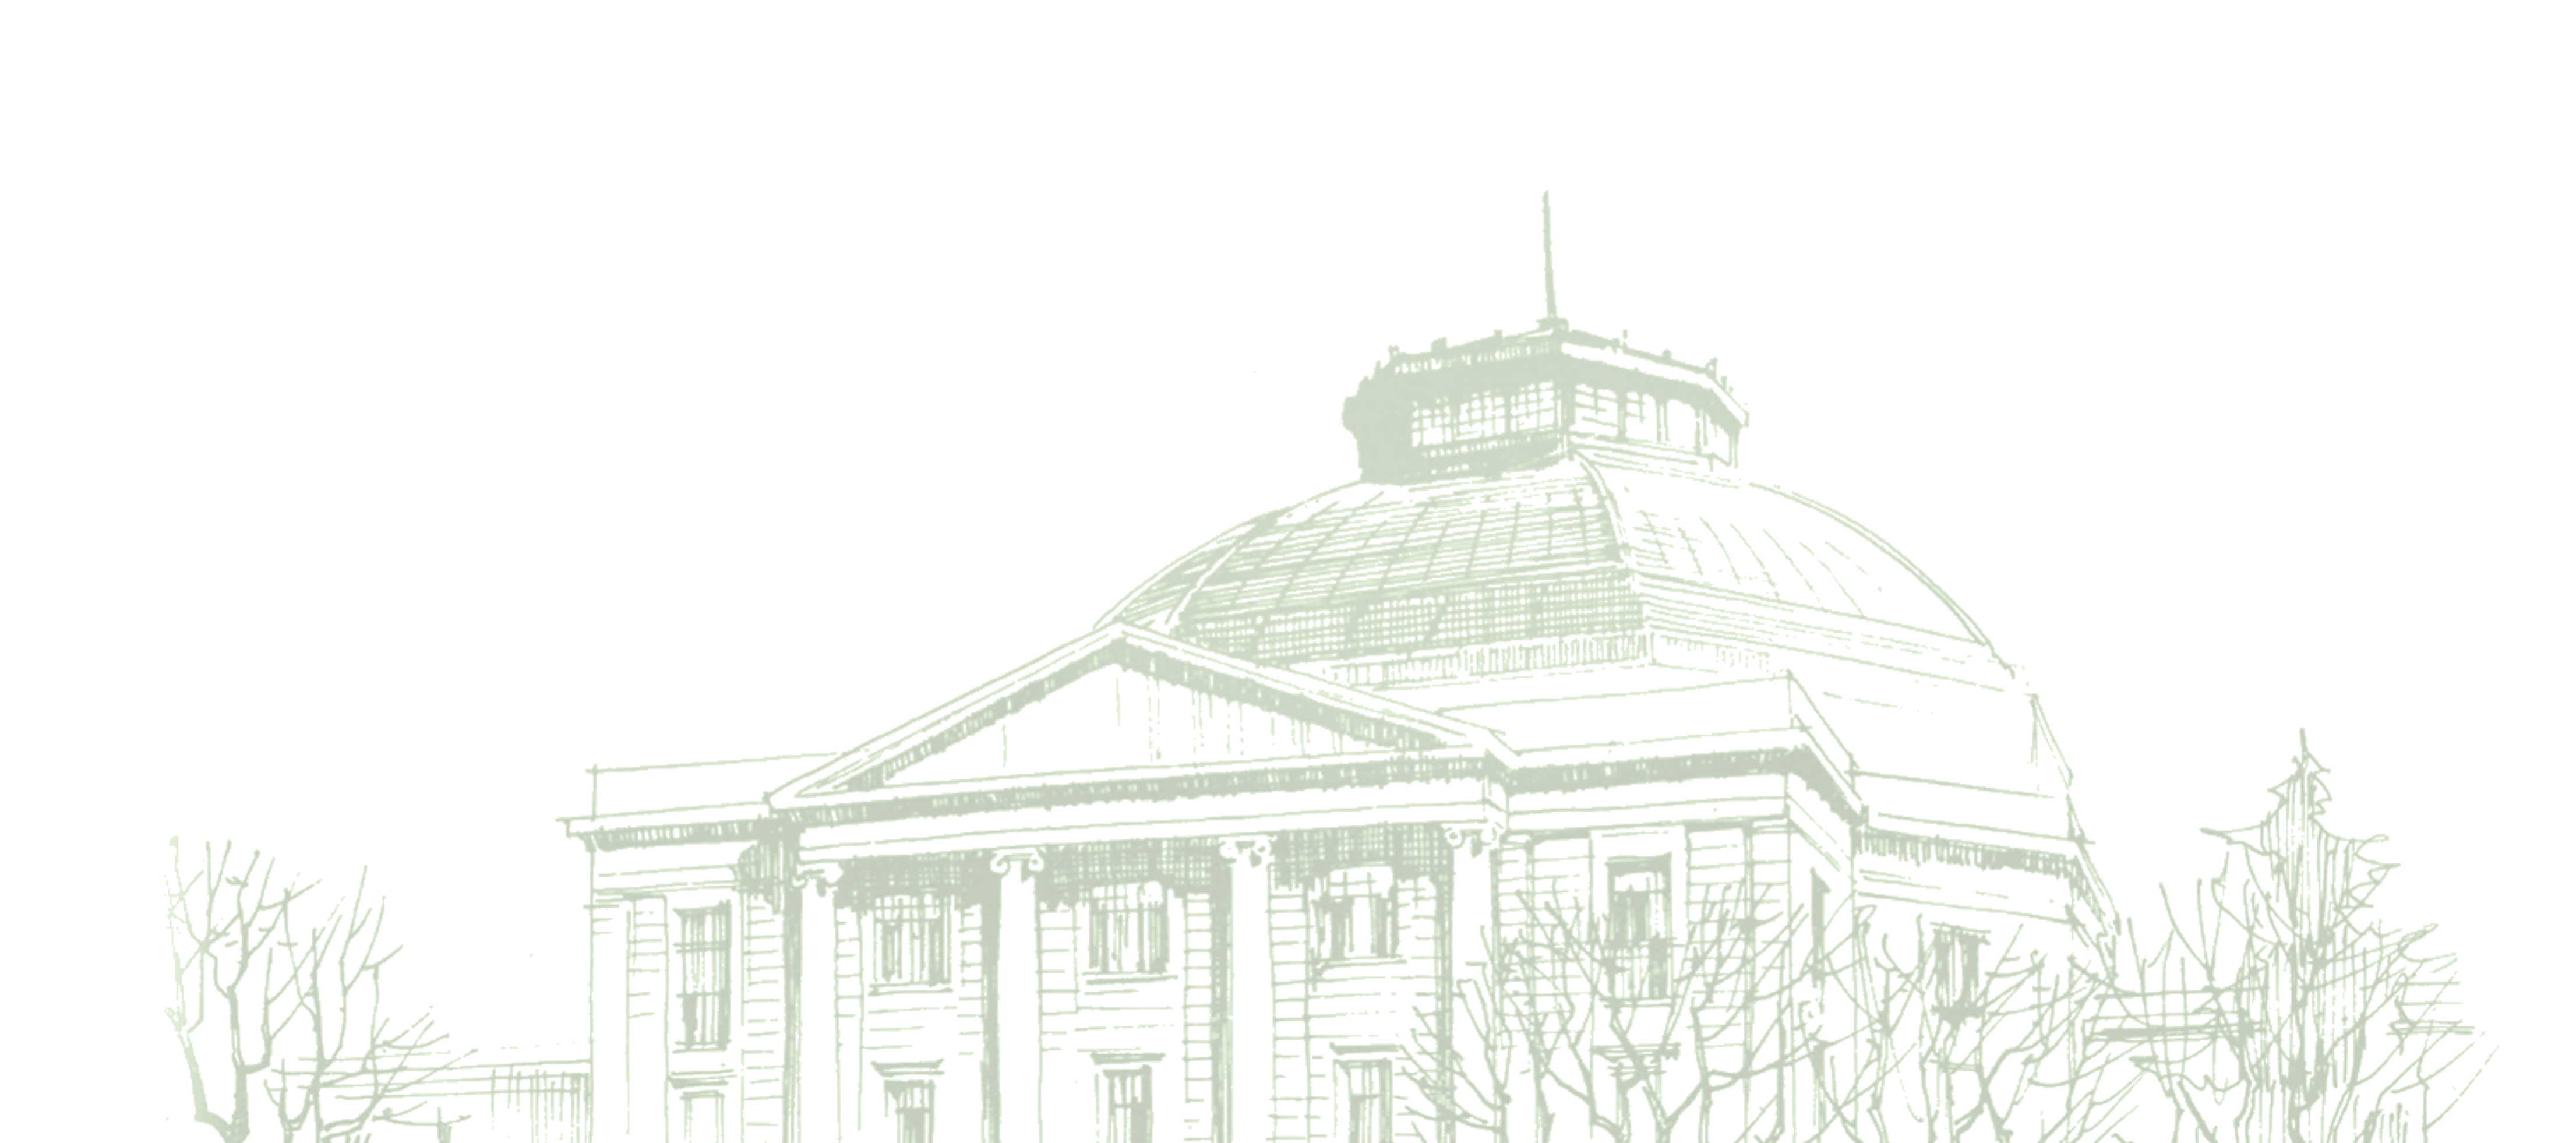
\includegraphics[width=.6\textwidth]{seu_building.png}
};
\node[above=0.5cm] at (current page.220){
    % \includegraphics[width=.25\textwidth]{logo_color_green.pdf}
    
\includegraphics[width=.13\textwidth]{SEUlogo.pdf}
    
\includegraphics[width=.13\textwidth]{RADIOlogo.pdf}
};
\end{tikzpicture}
}

\begin{document}
% 标题
\maketitle
%目录
\begin{frame}
    \frametitleb{目~录}
    \begin{minipage}{.45\linewidth}
        \begin{block}{\centering\small XXXXXXXX}
            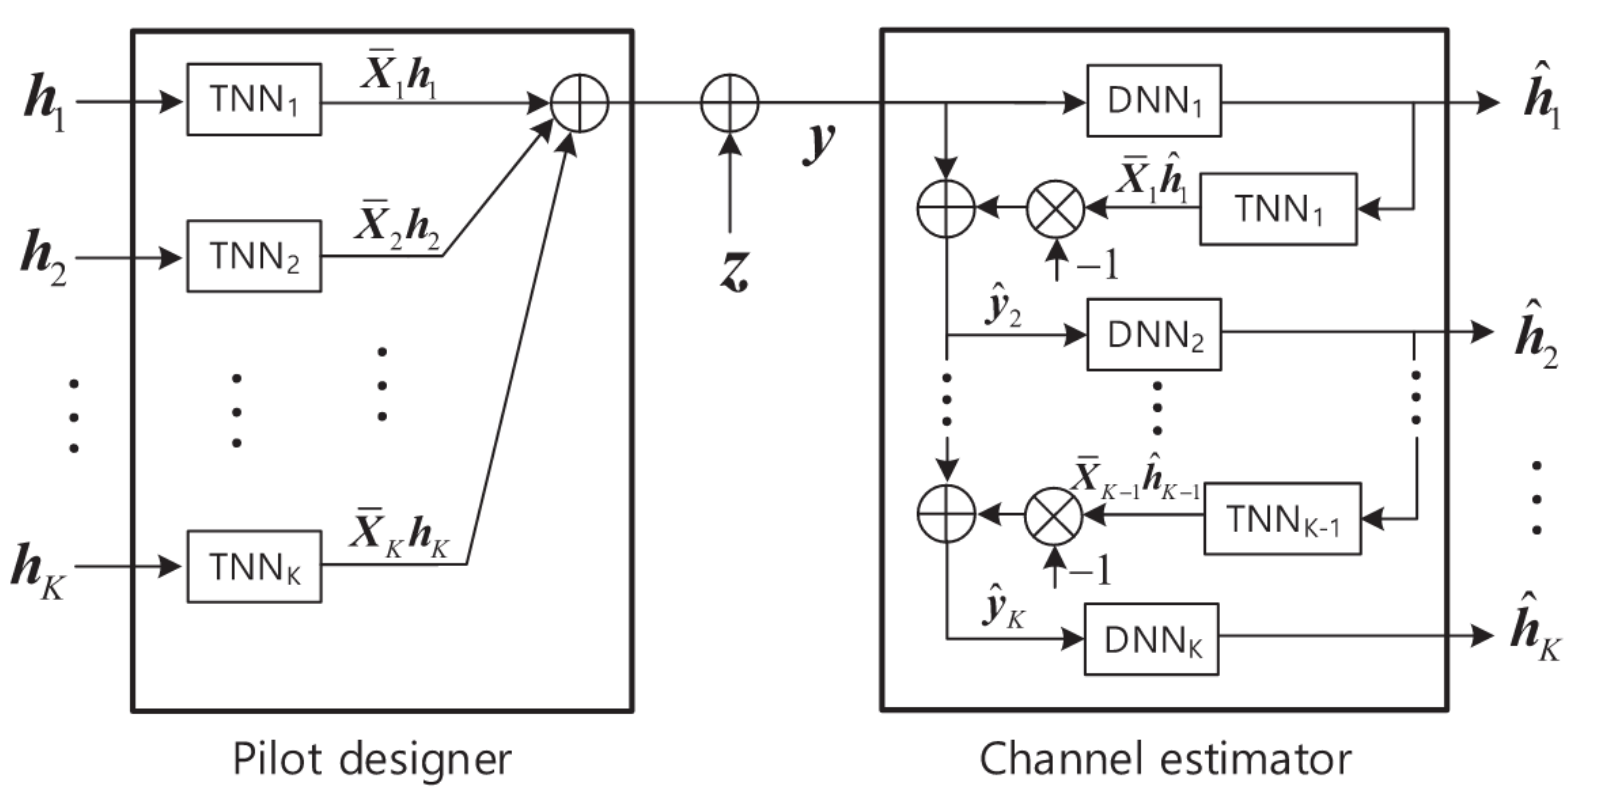
\includegraphics[width=\linewidth]{11-10.png}
            
            {\scriptsize *这边的图片插入去除背景的PDF会比较好。}
        \end{block}
    \end{minipage}\hfill
    \begin{minipage}
        {.47\linewidth}
        \tableofcontents[hideallsubsections] 
    \end{minipage}
    % \begin{multicols}{2}
    %    \tableofcontents
       % [pausesections]
       % You might wish to add the option 
    %  \end{multicols}

\end{frame}
% \faThList
% \part{testing}
\begin{frame}
    \frametitleb{基本说明}
    \begin{description}
        \item \emph{beamer比较适合于多公式、文字,少图表的情景。}
        \item [文档类] 中文beamer——\texttt{ctexbeamer}
        \item [尺寸] 16:9——\texttt{aspectratio=169}, 4:3——\texttt{aspectratio=43}
         \item [字体]使用非衬线体。中文思源黑体(常规)+{\XWWK{霞鹜文楷}}(斜体)、西文采用\LaTeX{}默认。
         \item [字体大小] 可选:10pt、11pt、12pt
        \item [颜色] 和\LaTeX{}撰写文档一致,多出\structure{结构色}等。
        \item [动画] 使用\texttt{\textbackslash pause}进行暂停。更复杂的可以看文档(命令行\texttt{texdoc beamer},网上也有中文版)
      
    \end{description}

\end{frame}


\section{文字与公式}
\subsection{文字的相关测试与样例}

\begin{frame}
    \frametitle{文字测试——原始标题样式}

    \begin{itemize}
        \item ABCD,东南大学信息学院,1234
        \item \textit{ABCD,东南大学信息学院,1234}
        \item \textbf{ABCD,东南大学信息学院,1234}
        \item \textbf{\textit{ABCD,东南大学信息学院,1234}}
        \item \emph{\textit{ABCD,东南大学信息学院,1234}}
    \end{itemize}

    \begin{enumerate}
        \item ABCD,东南大学信息学院,1234
        \item \textit{ABCD,东南大学信息学院,1234}
        \item \textbf{ABCD,东南大学信息学院,1234}
        \item \textbf{\textit{ABCD,东南大学信息学院,1234}}
        \item \emph{\textit{ABCD,东南大学信息学院,1234}}
    \end{enumerate}
\end{frame}

\begin{frame}
    \frametitleb{文字——多栏并排、东大信息标题样式}

    多栏并排,我一般是用\texttt{minipage}环境,方便调整列宽。

    \begin{minipage}
        {.27\textwidth}
        \begin{block}
            {}
            \centering 无序列表环境
        \end{block}
        \begin{itemize}
            \item 东南信息SEU4
            \item \textit{东南信息SEU4}
            \item \textbf{东南信息SEU4}
            \item \textbf{\textit{东南信息SEU4}}
            \item \emph{东南信息SEU4}
        \end{itemize}
    \end{minipage} 
    \begin{minipage}
        {.27\textwidth}
        \begin{block}
            {}
            \centering 有序列表环境
        \end{block}
        \begin{enumerate}
            \item 东南信息SEU4
            \item \textit{东南信息SEU4}
            \item \textbf{东南信息SEU4}
            \item \textbf{\textit{东南信息SEU4}}
            \item \emph{东南信息SEU4}
        \end{enumerate}
    \end{minipage} 
        \begin{minipage}
            {.35\textwidth}
        \begin{block}
            {}
            \centering description环境
        \end{block}
        \begin{description}
            \item[直立体] 东南信息SEU4
            \item[斜体] \textit{东南信息SEU4}
            \item[粗体] \textbf{东南信息SEU4}
            \item[粗斜体] \textbf{\textit{东南信息SEU4}}
            \item[强调] \emph{东南信息SEU4}
        \end{description}
    \end{minipage}

\end{frame}


\subsection{block的相关测试与样例}
\begin{frame}
    \frametitleb{三种block环境与一些标记}

    \begin{block}
        {基本block}
        采用东大标准绿色。
    \end{block}

    \begin{exampleblock}
        {举例block}
        采用黄色,左图右文混排我使用的是这个block。
    \end{exampleblock}

    \begin{alertblock}
        {重要block}
        采用红色。
    \end{alertblock}

    小图标采用\texttt{fontawesome5}宏包,主要使用箭头\faArrowCircleLeft、\faArrowCircleDown。
\end{frame}

\subsection{公式的相关测试与样例}
\begin{frame}
    \frametitleb{使用\texttt{annotate-equations}宏包为公式添加注释}

    请参考\href{https://github.com/st--/annotate-equations}{annotate-equations}宏包的使用说明。
    
    这里使用的颜色在beamercolorthemeSEUcolor.sty中定义。

    两步干扰消除:
    \begin{equation*}
        \mathbf Y    =\eqnmarkbox[SEUcolor]{nodeYp}{\sum_{u=1}^U \mathbf H_u  \sqrt{\rho} \, \mathrm{diag}(\mathbf p_u)} + \eqnmarkbox[SEUcolor]{nodeYd}{\sum_{u=1}^U \mathbf H_u \sqrt{1-\rho} \, \mathrm{diag}(\mathbf d_u) } + \mathbf N
    \end{equation*}
    \annotate{below,left}{nodeYp}{$\triangleq\mathbf Y_\text{p}$}
    \annotate{below,right}{nodeYd}{$\triangleq\mathbf Y_\text{d}$}


    软符号映射:
    \begin{equation*}
        [\hat{\mathbf{d}}]_u = \tikzmarknode{nodeSum}{\sum_{a\in\mathcal{Q}}} \eqnmarkbox[SEUdarkyellow]{nodeA}{a} \cdot \eqnmarkbox[SEUcolor]{nodeProb}{\mathbb{P}\left[[\mathbf{d}]_u = a \,|\, \mathsf{L}_\text{map}^A \right]}
    \end{equation*}
    \annotate[yshift=.7em,xshift=1em]{below,right}{nodeSum}{\scriptsize \textit{加权求和}}
    \annotate[yshift=.5em]{above}{nodeA}{\scriptsize \textit{星座点对应的复值符号}}
    \annotate{below}{nodeProb}{\scriptsize \textit{根据LLR得到的先验概率}}

    * 该页面目前仅在Mac\TeX{}~2025和Overleaf上测试。
\end{frame}

\section{图片混排}

\begin{frame}
    \frametitleb{图文混排测试1(带脚注)\emph{(Chu \textit{et al}., 2022)}\footnote{\fontsize{7pt}{7pt}\selectfont  M. Chu, A. Liu, V. K. N. Lau, C. Jiang, and T. Yang, “Deep Reinforcement Learning based End-to-end Multi-user Channel Prediction and Beamforming,” \textit{IEEE Trans. Wirel. Commun.}, pp. 1–1, 2022, doi: 10.1109/TWC.2022.3183255.}}
    
    \begin{itemize}
        \item 信道预测:利用已知的导频信号、接收到的导频$\mathbf Y$和一些历史信息\emph{直接预测实时下行链路 CSI},而不需要信道互易性。
        % \item 采用\emph{actor-critic方法}来解决连续空间的问题,actor网络直接输出policy,critic网络输出估计值函数来衡量动作的性能。
    \end{itemize}


    \begin{minipage}[m]{.47\textwidth}
     \begin{center}
        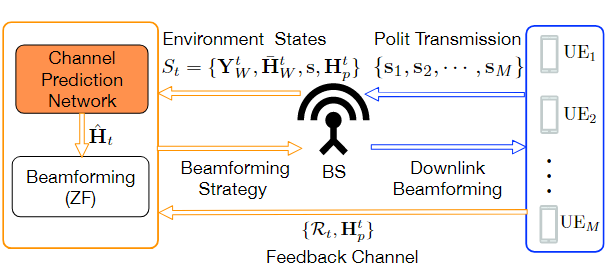
\includegraphics[width=\textwidth]{image-20221118100813715}
     \end{center} 
    \vspace{-10pt}每个用户每$W$个时隙发一次导频,在$W-1$个时隙BS都用这次预测的信道
    \end{minipage} 
    \begin{minipage}[m]{.47\textwidth}
    \begin{exampleblock}{}
    \raisebox{-1pt}{\structure{\faArrowCircleLeft}}\parbox{.95\textwidth}{\centering 优化目标}
    \end{exampleblock} 
    \begin{itemize}
        \item 和速率:$\mathcal{R}=\sum\limits_{i=1}^{M} r_{i}=\sum\limits_{i=1}^{M} B \log \left(1+\Upsilon_{i}\right)$
        \item (隐式)预测损失:$P^{\mathrm{loss}}=\sqrt{\sum\limits_{i=1}^{M}\left\|\mathbf{H}_{i}-\hat{\mathbf{H}}_{i}\right\|^{2}}$
    \end{itemize}
    \end{minipage}



\end{frame}

\begin{frame}
    \frametitleb{图文混排测试2\emph{(Chu \textit{et al}., 2022)}}
    
    \begin{itemize}
        % \item 信道预测:利用已知的导频信号、接收到的导频$\mathbf Y$和一些历史信息\emph{直接预测实时下行链路 CSI},而不需要信道互易性。
        \item 采用\emph{actor-critic方法}来解决连续空间的问题,actor网络直接输出policy,critic网络输出估计值函数来衡量动作的性能。
    \end{itemize}


    \begin{minipage}[m]{.47\textwidth}
     \begin{center}
        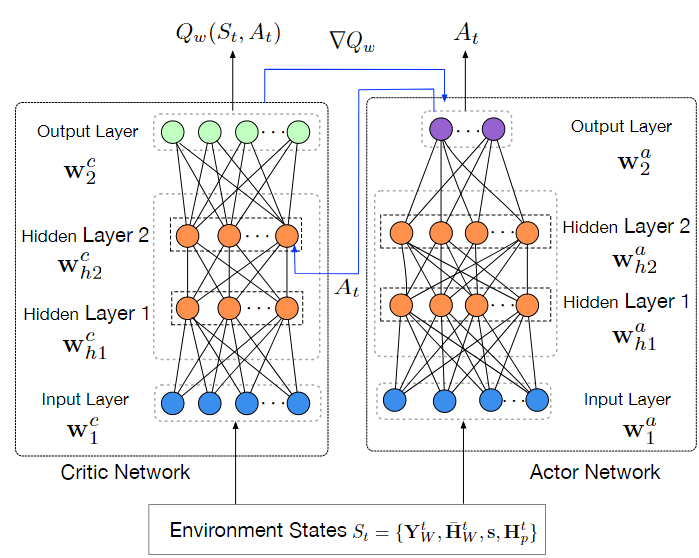
\includegraphics[width=.85\textwidth]{image-20221118101131606.png}
     \end{center} 
    \end{minipage} 
    \begin{minipage}[m]{.47\textwidth}
    \begin{exampleblock}{}
    \raisebox{-1pt}{\structure{\faArrowCircleLeft}}\parbox{.95\textwidth}{\centering 信道预测的DRL网络}
    \end{exampleblock} 
    状态:$S_{t}=\left\{\mathbf{Y}_{W}^{t}, \overline{\mathbf{H}}_{W}^{t}, \mathbf{s}, \mathbf{H}_{p}^{t}\right\}$
    \begin{itemize}
        \item $\mathbf Y_W^t$:上行链路导频接收信号的历史
        \item $\mathbf s$:导频
        \item $\bar{\mathbf H}_W^t$:信道的历史预测结果
        \item $\mathbf H_p^t = \mathbf H_{(t-\mod(t,W))}$:当前时隙遵循的信道估计反馈
    \end{itemize}
    \end{minipage}

\end{frame}



\begin{frame}
    \frametitleb{左右双图与block内的脚注\emph{(Kang \textit{et al}., 2020)}\footnote{\fontsize{7pt}{7pt}\selectfont  J. -M. Kang, I. -M. Kim and C. -J. Chun, "Deep Learning-Based MIMO-NOMA With Imperfect SIC Decoding," in \textit{IEEE Systems Journal}, vol. 14, no. 3, pp. 3414-3417, Sept. 2020, doi: 10.1109/JSYST.2019.2937463.}}

 
    \begin{minipage}[t]{.47\textwidth}


        场景:\emph{上行链路} $K$个用户,基站$N$天线。
        
        \vspace{10pt}
        \centering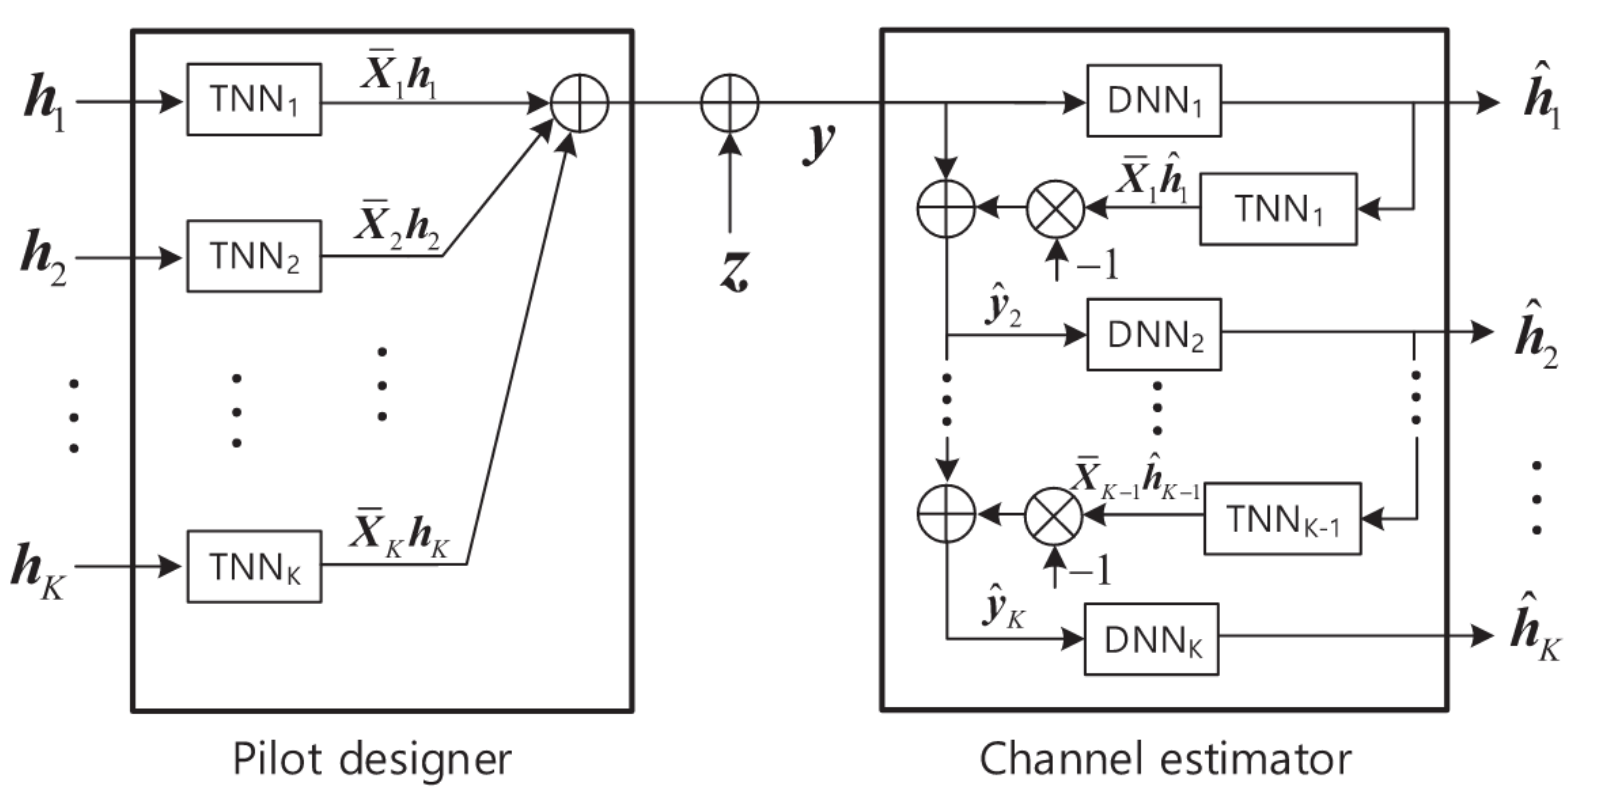
\includegraphics[height=.4\textheight]{11-10.png}
        \vspace{-5pt}\begin{exampleblock}{}
            \centering{导频设计和SIC信道估计}\emph{(Chun \textit{et al}., 2019)\footnotemark}
        \end{exampleblock}
    \end{minipage}\footnotetext{\fontsize{7pt}{7pt}\selectfont C.-J. Chun, J.-M. Kang, and I.-M. Kim, “Deep Learning-Based Joint Pilot Design and Channel Estimation for Multiuser MIMO Channels,” \textit{IEEE Commun. Lett.}, vol. 23, no. 11, pp. 1999–2003, Nov. 2019, doi: 10.1109/LCOMM.2019.2937488.} \pause
    \begin{minipage}[t]{.47\textwidth}


        场景:\emph{下行链路} $K$个用户,基站$M$天线。
        
        \vspace{10pt}
        \centering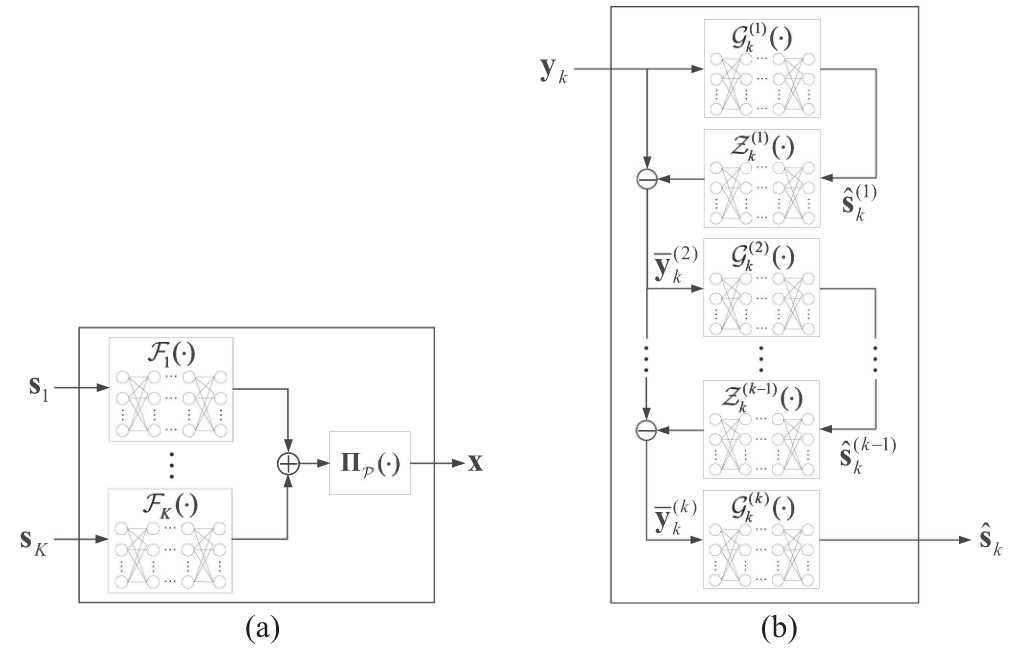
\includegraphics[height=.4\textheight]{image-20221118204141005.png}
        \vspace{-5pt}\begin{exampleblock}{}
            \centering{预编码和SIC信号检测}\emph{(Kang \textit{et al}., 2020)}
        \end{exampleblock}
    \end{minipage}
    
\end{frame}


\begin{frame}
    \frametitleb{轮换图片\emph{(Wang \textit{et al}., 2021)}\footnote{\fontsize{7pt}{7pt}\selectfont  X. Wang, P. Zhu, D. Li, Y. Xu and X. You, "Pilot-Assisted SIMO-NOMA Signal Detection With Learnable Successive Interference Cancellation," in \textit{IEEE Communications Letters}, vol. 25, no. 7, pp. 2385-2389, July 2021, doi: 10.1109/LCOMM.2021.3070705.}}

    场景:基站$N_r$个天线,$K$个单天线用户的上行链路SIMO系统,结合可训练投影梯度检测器(TPG),设计了一种导频辅助的可学习SIC接收机(PA-LSIC),\emph{充分控制每次迭代的步长}。

    \begin{minipage}[m]{.55\textwidth}
    \centering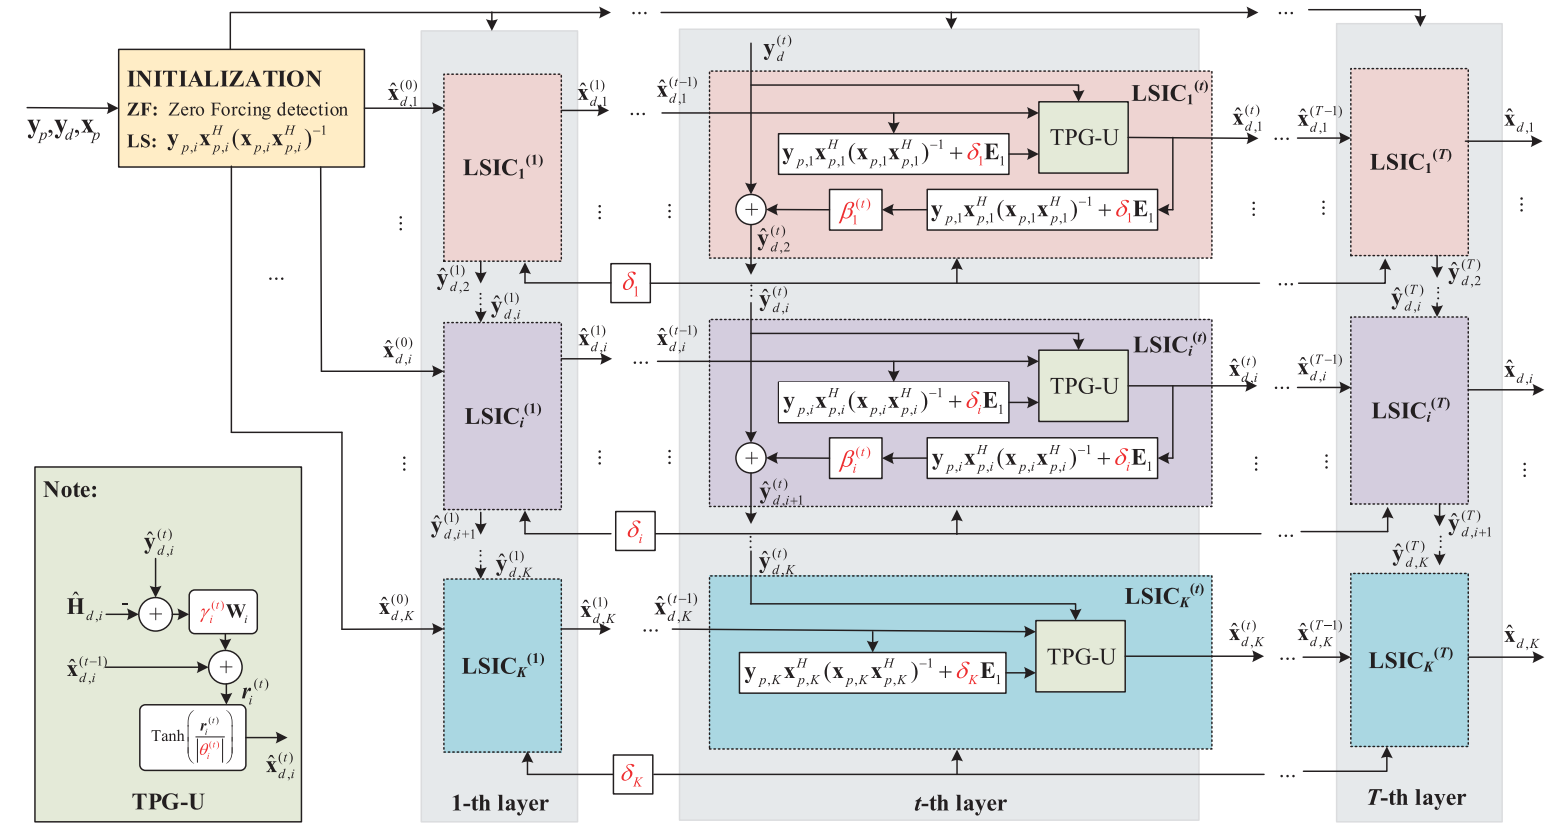
\includegraphics[width=\textwidth]{image-20221122195131349.png}
    \end{minipage} 
    \begin{minipage}[m]{.4\textwidth}
    \begin{overprint}
        \onslide<2>
        \begin{exampleblock}{}
            \raisebox{-1pt}{\structure{\faArrowCircleLeft}}\parbox{.95\textwidth}{\centering LSIC${}_{i}^{(t)}$块输入}
            \end{exampleblock} 
            \begin{itemize}
                \item {上轮迭代估计信号}:$\hat{\mathbf x}_{d,i}^{(t-1)}$
                \item {用户$i-1$第$t$轮迭代结束}\\ 
                \vspace{5pt}$\hat{\mathbf{y}}_{d, i}^{(t)}=\hat{\mathbf{y}}_{d}-\sum\limits_{j=1}^{i-1} \emph{\underline{\beta_{j-1}^{(t)}}} \widehat{\mathbf{H}}_{j} \hat{\mathbf{x}}_{d, j-1}^{(t)}$
                \item \vspace{1pt}{用户$i$导频LS信道估计}\\
                \vspace{3pt}$\widehat{\mathbf{H}}_{i}=\mathbf{y}_{p, i} \mathbf{x}_{p, i}^{H}\left(\mathbf{x}_{p, i} \mathbf{x}_{p, i}^{H}\right)^{-1}+\emph{\underline{\delta_{i} }} \mathbf{E}_{1}$
            \end{itemize}
        \onslide<3>
        \begin{exampleblock}{}
            \raisebox{-1pt}{\structure{\faArrowCircleLeft}}\parbox{.95\textwidth}{\centering TPG-U}
            \end{exampleblock} 
            \begin{itemize}
                \item \emph{梯度下降}\\
                    $\boldsymbol{r}_{i}^{(t)}  =\hat{\mathbf{x}}_{d, i}^{(t-1)}+\emph{\underline{\gamma_{i}^{(t)}}} \mathbf{W}_{i}\left(\hat{\mathbf{y}}_{d, i}^{(t)}-\widehat{\mathbf{H}}_{i} \hat{\mathbf{x}}_{d, i}^{(t-1)}\right) $\\
                    {\small 权重$\mathbf{W}_{i}=\widehat{\mathbf{H}}_{i}^{H}\left(\widehat{\mathbf{H}}_{i} \widehat{\mathbf{H}}_{i}^{H}+\emph{\underline{\xi_{i} }}\mathbf{I}\right)^{-1}$}
                \item \emph{投影}\\
                    $\hat{\mathbf{x}}_{d, i}^{(t)}  =\operatorname{Tanh}\left(\boldsymbol{r}_{i}^{(t)} /\left|\emph{\underline{\theta_{i}^{(t)}}}\right|\right)$
            \end{itemize}
    \end{overprint}
    
    \end{minipage}

\end{frame}

\begin{frame}
    \frametitleb{双栏 \emph{(刘雪骢, 2021)}\footnote{\fontsize{7pt}{7pt}\selectfont 刘雪骢. 基于深度学习的迭代MIMO检测算法研究[D].东南大学, 2021. DOI:10.27014/d.cnki.gdnau.2021.001889.}}                

    DetNet通过展开每一次梯度下降,来模拟迭代。

    \vspace{-15pt}\begin{minipage}[t]{.47\textwidth}
        \begin{exampleblock}{}
            \raisebox{-1pt}{\structure{\faArrowCircleDown}}\parbox{.95\textwidth}{\centering DetNet的单层结构}
            \end{exampleblock} 
        通过ML检测的梯度下降投影形式
        \[\hat{x}_{k+1}=\prod\left[\hat x_k+\delta_kH^Hy+\delta_kH^H\hat x_k\right]\]
    \begin{center}
        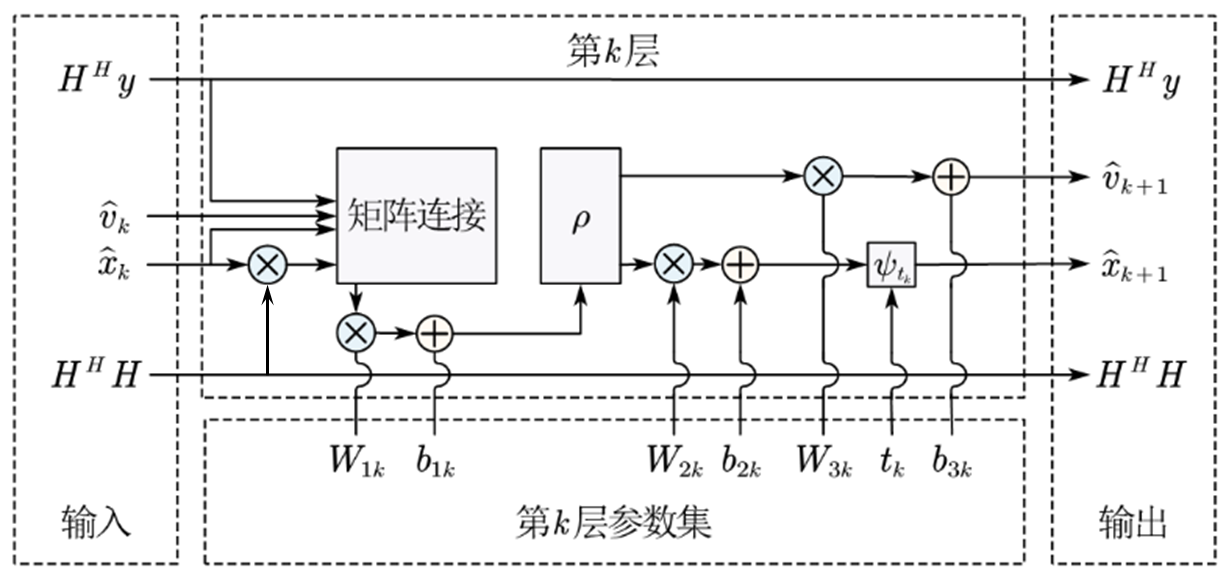
\includegraphics[width=.8\textwidth]{image-20221202134626792.png}
    \end{center}
    \end{minipage} 
    \begin{minipage}[t]{.47\textwidth}
    \begin{exampleblock}{}
        \raisebox{-1pt}{\structure{\faArrowCircleDown}}\parbox{.95\textwidth}{\centering DetNet的软输出改造(?)}
    \end{exampleblock} 
    \[\begin{aligned}
        \operatorname{LLR}(\widehat{x}) =&\ln \frac{P\left(b_{i}=1 \mid \widehat{x}\right)}{P\left(b_{i}=0 \mid \widehat{x}\right)} \\
 \approx &\ln \frac{\left.\min \left\{d_{E u c}\left(x_{i}, c_{k, i}^{0}\right)\right\}\right|_{k=1} ^{\log _{2}(M)}}{\left.\min \left\{d_{E u c}\left(x_{i}, c_{k, i}^{1}\right)\right\}\right|_{k=1} ^{\log _{2}(M)}}
    \end{aligned}\]

    其中,$c_{k,i}^0$表示在星座图中第$i$个比特是 0 的第$k$个星座点
    \end{minipage}
\end{frame}

\begin{frame}
    \frametitleb{TikZ图片与上下布局}

    \begin{center}
        \scriptsize
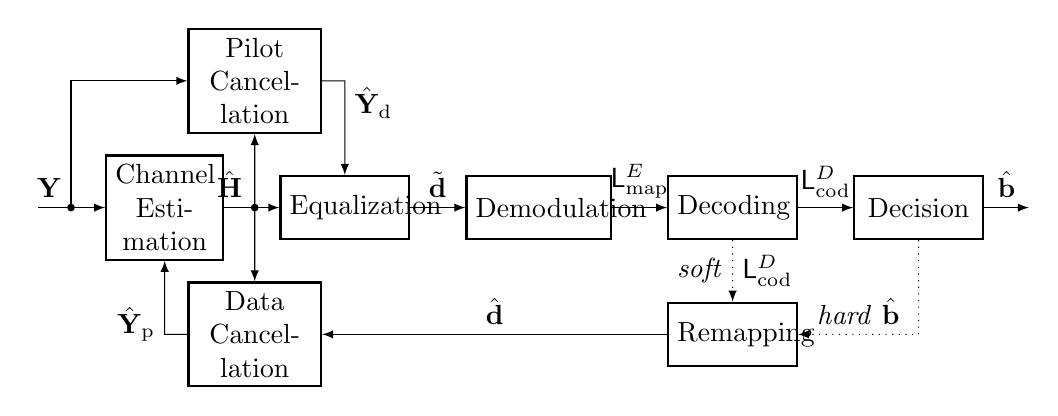
\begin{tikzpicture}  [scale=.7,node distance=0.7cm]
\node[block,text width=1.25cm] (a) {Channel Estimation};  
\draw[latex-] (a) -- node[above left]{$\mb Y$} +(-2.3cm,0);
\node[block,right=of a,text width=1.4cm] (b) {Equalization};   
\node[block,right=of b,text width=1.6cm] (c) {Demodulation};  
\node[block,right=of c] (d) {Decoding};
\node[block,right=of d] (e) {Decision};
\fill ($(a)!0.5!(b)$) circle[radius=2pt];
\node[block,text width=1.45cm] (f) at ([yshift=2.3cm]$(a)!0.5!(b)$) {Pilot Cancellation};  
\node[block,text width=1.45cm] (g) at ([yshift=-2.3cm]$(a)!0.5!(b)$) {Data Cancellation};
\node[block] (h) at ([yshift=-2.3cm]$(d)$) {Remapping};  
\coordinate (ii) at ([xshift=-1.7cm]$(a)$) ;  
\fill (ii) circle[radius=2pt];
% \node[draw, fill opacity=0.5,inner xsep=5mm,inner  
%      ysep=6mm,fit=(d)(e),label={130:A}](f){}; % 这里的 label 命令用于标记块,它涵盖了块 D 和 E。 
\draw[line] (a)--  node[above left]{$\hat{\mb H}$} (b);  
\draw[line] (b)-- node[above]{$\tilde{\mb d}$}(c);  
\draw[line] (c)-- node[above]{$\mathsf{L}_\text{map}^E$}(d); 
\draw[line] (d)-- node[above]{$\mathsf{L}_\text{cod}^D$}(e);
\draw[line,dotted] (d)-- node[right]{$\mathsf{L}_\text{cod}^D$}node[left]{\textit{soft}}(h);
\draw[line,dotted] (e)--(e |- h) -> node[above]{\textit{hard}  $\hat{\mb b}$}(h);
\draw[line] (h)--node[above]{$\hat{\mb d}$} (g);  
\draw[line] ($(a)!0.5!(b)$)-- (g);  
\draw[line] ($(a)!0.5!(b)$)-- (f);  
\draw[line] (e) -- node[above]{$\hat{\mb b}$} ++(2cm,0);
\draw[line] (g) -- (g -| a) ->  node[below left]{$\hat{\mb Y}_\text{p}$} (a); %
\draw[line] (ii) -- (ii |- f) -> (f);
\draw[line] (f) -- (f -| b) ->node[above right]{$\hat{\mb Y}_\text{d}$}  (b); % 
% \draw[line] (d)-- ($(a)!0.5!(b)$);  
\end{tikzpicture}  

{\small \emph{Fig. 3.} Block diagram of SIP iterative receiver.}
    \end{center}

    \begin{multicols}{2}
        \begin{itemize}
            \item 考虑\emph{信道估计}和两次\emph{干扰消除}
            \begin{itemize}
                \item 信道估计前——数据干扰消除,得$\hat{\mb Y}_\text{p}$
                \item 均衡前——导频干扰消除,得$\hat{\mb Y}_\text{d}$
            \end{itemize}
            \item 总体思想:\emph{判决反馈}
            \begin{itemize}
                \item 利用迭代中的LLR,逐步增强信道估计和数据检测,消除叠加的影响
            \end{itemize}
        \end{itemize}
    \end{multicols}

\end{frame}

\section{硕士期间成果}
\begin{frame}
    \frametitleb{硕士期间成果}

    \begin{block}{}
        \bfseries\structure{\faScroll ~~论文}
    \end{block}

    {\small \begin{enumerate}
        \item \textbf{XX X}, XX X, XX X, XX X and XX X. Enhancing xxxx xxxx xxx[J]. \textbf{\itshape IEEE Wireless Communications Letters}, 2024, 13(x): xxxx-xxxx.
        \item XX X, XX X, \textbf{XX X}, XX X and XX X. xxxx xxxx xxx[J]. \textbf{\itshape IEEE XXXX XXXX}, XXXX, XX(xx): xxxx-xxxx.
    \end{enumerate}}

    \begin{block}{}
        \bfseries\structure{\faNetworkWired ~~科研项目}
    \end{block}
    {\small\begin{itemize}
        \item XXXXXXXXX,东南大学与XX公司合作项目,20XX.XX -- 20XX.XX. \\(已结题,负责算法设计与实现)
    \end{itemize}}

\end{frame}

\section{补充说明与参考资料}
\begin{frame}
\frametitleb{补充说明}
    \begin{itemize}
        \item 经过测试,该模板直接上传Overleaf或\TeX{}Live~2022或Mac\TeX{}~2025均可运行,其他版本未测试。
        \begin{itemize}
            \item Overleaf请使用XeLaTeX编译器进行编译。
            \item 本地\TeX{}Live或Mac\TeX{}请使用XeLaTeX编译器编译两遍。
        \end{itemize}        
        \item 请勿删除\texttt{fonts}文件夹,此文件夹内为模板中使用的中文字体。更纱黑体、霞鹜文楷均为可商用字体(来源:Github、猫啃网)。本地可以直接安装使用。其余字体问题可参考“\href{https://levitate-qian.github.io/2022/04/14/latex-note-04/}{LaTeX札记(四):字体}”。
        \item 请勿删除\texttt{SEU\_RADIO\_image}文件夹,此文件夹内为模板中使用的东大信息相关图片。
        \item 图片请放置在\texttt{image}文件夹下,或采用其他相对路径
    \end{itemize}
\end{frame}

\begin{frame}
    \frametitleb{参考资料}

        \begin{alertblock}{强烈推荐}
            \begin{itemize}
                \item 一份(不太)简短的\LaTeXe 介绍 (最新是6.0.5版本) \url{https://mirrors.tuna.tsinghua.edu.cn/CTAN/info/lshort/chinese/}
                \item 中文版beamer宏包手册:\href{http://static.latexstudio.net/wp-content/uploads/2017/02/BeamerUserGuide_V3.24_zh-cn.pdf}{BeamerUserGuide V3.24 zh-cn}
            \end{itemize}
        \end{alertblock}

        \begin{block}{推荐}
            \begin{enumerate}
                \item \LaTeX 入门, 刘海洋, 电子工业出版社, 2013.(内容比lshort多一点,但也是工具书的性质)
                \item \href{https://math.ecnu.edu.cn/~jypan/Latex/index.html}{\LaTeX 科技排版}:华师大老师的网站,主要是讲座的beamer  
            \end{enumerate}
            
        \end{block}
        \begin{exampleblock}
            {我自己一些拙劣的整理}
            \begin{itemize}
                \item \href{https://levitate-qian.github.io/categories/LaTeX-and/}{LaTeX归档}(其中,“\href{https://levitate-qian.github.io/2020/12/01/latex-lecture/}{LaTeX模板分享}”里面有一些整理)
            \end{itemize}
        \end{exampleblock}
\end{frame}



%Q&A
\section*{Q\&A}
\begin{frame}
    \centering
    \vspace{2.2cm}

    \structure{\fontsize{30pt}{35pt}\selectfont\textbf{Q{\Huge\&}A}}

    \vspace{0.4cm}{\Large\itshape \faSlideshare~希望各位老师批评指正!}

    \vspace{1.3cm}
    \begin{minipage}[m]{.65\textwidth}
        \centering
       \begin{block}{}
        \begin{minipage}[m]{.15\textwidth}
            
\includegraphics[width=\textwidth]{SEUlogo.pdf}
        \end{minipage}
        \begin{minipage}[m]{.67\textwidth}
     \small\centering
    \inserttitle

    \textbf{王东南}(220000)
    
    {指导老师:\textbf{王东}~教授}
    \end{minipage}
    \begin{minipage}[m]{.15\textwidth}
        
\includegraphics[width=\textwidth]{RADIOlogo.pdf}
    \end{minipage}
    \end{block} 
    \end{minipage}
    
    
\end{frame}
\end{document}
